\chapter{Development Guide}

\section{Workflow}

\section{Developing}

\subsection{Advanced PHP Tips}
\subsubsection{String Equals Zero In PHP}
\footnote{Original text from: \url{http://www.hashbangcode.com/blog/string-equals-zero-php}}Due to the weakly-typed nature of PHP you can do some odd things, some of which are good, and some of which will enable you to shoot yourself in the foot. Care if you compare string with integer values. Take the following little snippet.

%\fvset{frame=single}
%\begin{pyglist}[language=php,numbers=left,numbersep=5pt]
%<?php
%$index = 0;
%var_dump($index == 'attributes'); //>bool(true)
%\end{pyglist}
%\fvset{frame=none}

Maybe you expect that the in-built function var\_dump() outputs bool(false) because 0 is not equal 'attributes' but instead the result is bool(true)! When you compare an integer and string, PHP converts the string to an integer. The integer of the string 'attributes' is 0. So var\_dump(0 == 0) outputs bool(true).

\section{Integration}

\subsection{Reviewing}

As a reviewer one has the responsibility of ensuring code quality. The Gerrit plugin offers many features which make this process easier. To open the Gerrit plugin's interface click on the icon on the bottom edge of the PHPStorm interface, as in \figref{fig:gerrit-plugin-interface}.

\newpage

\begin{figure}[h] 
	\centering
	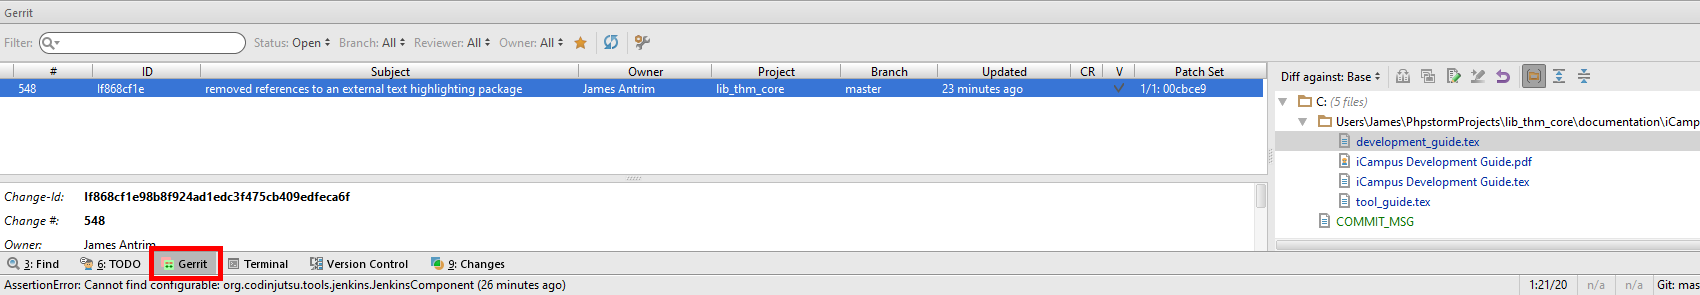
\includegraphics[width=14cm]{gerrit-plugin-interface.png}
	\caption{Gerrit Plugin Interface}
	\label{fig:gerrit-plugin-interface}
\end{figure}

\noindent
In this figure we see a previous commit already highlighted. This commit has already been examined by Jenkins and has been deemed to be of acceptable quality, this is evinced by the checkmark in the 'v' column. Jenkins can only performs automated tests and checks, which are good for problems which can be detected in this manner. It cannot find every error, and it is this point which the review system seeks to iron out, letting reviewers examine code before it is permanently made of a release.\\
\\
Because it is highlighted, the files changed by this commit are listed on the right hand side. To see the changes to individual files right click on the file in this list and select \texttt{Show Diff}.\\

\begin{figure}[h] 
	\centering
	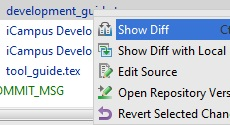
\includegraphics[width=6cm]{gerrit-plugin-file-review.png}
	\caption{File Review Interface}
	\label{fig:gerrit-plugin-file-review}
\end{figure}

\noindent
This opens a further interface where the local contents are then compared with those in the change. A review can then examine changes line by line to ensure the desired code quality has been reached. At this point multiple options open, but only the most important will be described.\\

\subsubsection{Approval}

Should the code be of an acceptable quality the reviewer can merge the commit with the master branch by right clicking on the list entry, opening the context menu (\figref{fig:gerrit-plugin-context-menu}). Then the reviewer can 'review' the commit by hovering over the word \texttt{Review} to the right a sub menu opens in which he selects \texttt{$+2$}. This tells Gerrit that the code has been reviewed and approved. By right-clicking again on the entry and left-clicking on submit the commit will then be merged into the master branch.

\begin{figure}[h] 
	\centering
	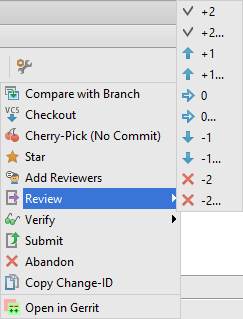
\includegraphics[width=5cm]{gerrit-plugin-context-menu.png}
	\caption{Commit Context Interface}
	\label{fig:gerrit-plugin-context-menu}
\end{figure}

\subsubsection{Rejection}

If the code needs improvement it can either be rejected outright or fixed. Outright rejection is performed over the same context menu as approval, only instead of \texttt{$+2$}, the reviewer then selects \texttt{$-2$} or \texttt{$-2$...}. The second option allows for a rejection message, which can be useful for stating the reason why the commit was rejected.\\
\\
The other option is to correct or improve the commit. To do so, the reviewer opens the commit context menu and selects \texttt{Checkout}. This creates a new local branch with the same stand as the commit to be corrected or improved. In the bottom right hand corner of the PhpStorm interface the new branch is now displayed. Click on the branch name to open the branch-interface. Select master and in the context menu that opens select \texttt{Checkout}. This sets your repository to the stand of the current master branch. Next reopen the branch-interface and click on the newly created local branch. In the menu that now opens select \texttt{Merge}. This merges that changes from the new branch onto the stand of the master.\\
\\
Now that you have the commit's changes in your master branch proceed to correct and improve the changed files as appropriate. When you have completed your changes append them to the previous commit by placing the checkmark in the \texttt{Append Commit} box and performing the commit and push as you normally would.
